\documentclass[11pt,aspectratio=169]{beamer}

\usepackage{amsmath,amssymb,bm}
\usepackage{booktabs}
\usepackage{tikz}
\usetikzlibrary{arrows.meta,positioning,calc}

\usetheme{default}
\setbeamertemplate{navigation symbols}{}
\setbeamertemplate{headline}{}
\setbeamertemplate{footline}{%
  \leavevmode
  \hbox{%
    \begin{beamercolorbox}[wd=\paperwidth,ht=2.6ex,dp=1.1ex,right]{page number in head/foot}%
      \insertframenumber/\inserttotalframenumber\hspace{0.35cm}
    \end{beamercolorbox}%
  }%
}
\setbeamertemplate{frametitle}{\vspace{0.25cm}\insertframetitle\par\vspace{0.08cm}\hrule}
\setbeamercolor{normal text}{fg=black,bg=white}
\setbeamercolor{frametitle}{fg=black,bg=white}
\setbeamercolor{structure}{fg=black}
\setbeamersize{text margin left=0.7cm,text margin right=0.7cm}

\newcommand{\dd}{\,\mathrm{d}}
\newcommand{\Om}{\Omega}
\newcommand{\GamD}{\Gamma_D}
\newcommand{\GamN}{\Gamma_N}
\newcommand{\Th}{\mathcal T_h}
\newcommand{\Fh}{\mathcal F_h}
\newcommand{\Vzero}{\mathcal V_0}
\newcommand{\Vhzero}{\mathcal V_{h,0}}
\newcommand{\Qh}{\mathcal Q_h}
\newcommand{\norm}[2][]{\left\lVert#2\right\rVert_{#1}}
\newcommand{\seminorm}[2][]{\left\lvert#2\right\rvert_{#1}}
\newcommand{\grad}{\nabla}
\newcommand{\divg}{\nabla\!\cdot}
\newcommand{\bn}{\bm n}
\newcommand{\bq}{\bm q}

\begin{document}

\begin{frame}[plain]
  \centering\vfill
  {\LARGE\bfseries A Posteriori Error Estimation\par}
  \vspace{0.45cm}
  {\large Residual functional and elementwise localization\par}
  \vfill
\end{frame}

\begin{frame}{Lecture outline}
This lecture begins with the finite element solution already computed.

\begin{enumerate}
  \item Define its residual and connect the residual to the unknown error.
  \item Explain why the exact residual identity is not yet computable.
  \item Introduce mesh facets, normals, and normal-flux jumps.
  \item Begin localization by integrating by parts on each element.
\end{enumerate}

\vspace{0.35cm}
This begins the \emph{estimate} step of
\[
  \text{solve}\ \longrightarrow\ \text{estimate}\ \longrightarrow\
  \text{mark}\ \longrightarrow\ \text{refine}.
\]
The next lecture completes the residual representation and constructs the
computable estimator.
\end{frame}

\section{Residual and error}

\begin{frame}[plain]
  \centering\vfill
  {\LARGE\bfseries Residual and error\par}
  \vspace{0.4cm}
  {\large What can be computed after the finite element solve?\par}
  \vfill
\end{frame}

\begin{frame}{From an a priori rate to an a posteriori estimate}
Chapter 7 established an a priori estimate of the form
\[
  \norm[a]{u-u_h}
  \leq C_I\sqrt{k_1}\,h^{s-1}\seminorm[H^s(\Om)]{u}.
\]

It predicts how the error should decrease under uniform refinement, provided
the exact solution has the assumed regularity. It does not directly determine

\begin{itemize}
  \item the error in the solution already computed, because
  $\seminorm[H^s(\Om)]{u}$ is unknown; or
  \item which elements contribute most to that error, because the estimate
  contains the global mesh size $h$.
\end{itemize}

\vspace{0.2cm}
An a posteriori estimate replaces the unknown higher derivatives of $u$ by
quantities computed from $u_h$ and the prescribed data.
\end{frame}

\begin{frame}{Recall the continuous and discrete diffusion problems}
With $\bq=k\grad u$ and $q=\bq\cdot\bn$, define
\[
  a(w,v)=\int_\Om k\grad w\cdot\grad v\,\dd x,
  \qquad
  \ell(v)=\int_\Om fv\,\dd x+\int_{\GamN}qv\,\dd s.
\]
The exact solution satisfies
\[
  a(u,v)=\ell(v)
  \qquad\forall v\in\Vzero,
\]
whereas the finite element solution satisfies
\[
  a(u_h,v_h)=\ell(v_h)
  \qquad\forall v_h\in\Vhzero\subset\Vzero.
\]

\vspace{0.2cm}
Both equations use the same forms. Their difference is the set of test
functions: the discrete equations test only with functions in $\Vhzero$.
\end{frame}

\begin{frame}{The residual measures what the discrete equations do not test}
For any $v\in\Vzero$, define
\[
  \boxed{R(u_h;v)=\ell(v)-a(u_h,v).}
\]
This number is computable from $u_h$, $k$, $f$, and $q$ for any selected test
function $v$.

\vspace{0.25cm}
The exact equation gives $\ell(v)=a(u,v)$, so with $e=u-u_h$,
\[
\begin{aligned}
  R(u_h;v)
  &=a(u,v)-a(u_h,v)\\
  &=a(u-u_h,v)\\
  &=\boxed{a(e,v)}.
\end{aligned}
\]

For $v_h\in\Vhzero$, the discrete equation gives
\[
  R(u_h;v_h)=0.
\]
Thus the residual vanishes on the discrete test space, but generally not on
all of $\Vzero$.
\end{frame}

\begin{frame}{The residual dual norm equals the energy error}
Because $a(\cdot,\cdot)$ is an inner product on $\Vzero$,
\[
  |R(u_h;v)|=|a(e,v)|
  \leq \norm[a]{e}\,\norm[a]{v}.
\]
Dividing by $\norm[a]{v}$ and taking the supremum gives
\[
  \sup_{0\neq v\in\Vzero}
  \frac{|R(u_h;v)|}{\norm[a]{v}}
  \leq \norm[a]{e}.
\]

If $e\neq0$, choose $v=e$. Then
\[
  \frac{|R(u_h;e)|}{\norm[a]{e}}
  =\frac{a(e,e)}{\norm[a]{e}}
  =\norm[a]{e}.
\]
Therefore
\[
  \boxed{
  \norm[a]{u-u_h}
  =\sup_{0\neq v\in\Vzero}
  \frac{|R(u_h;v)|}{\norm[a]{v}}.}
\]
\end{frame}

\begin{frame}{Why the exact residual identity is not yet computable}
The identity
\[
  \norm[a]{e}
  =\sup_{0\neq v\in\Vzero}
  \frac{|R(u_h;v)|}{\norm[a]{v}}
\]
is exact, but it is not yet an estimator that can be evaluated:

\begin{enumerate}
  \item the supremum ranges over the infinite-dimensional space $\Vzero$;
  \item equality is attained in the unknown direction $v=e$; and
  \item the resulting single number does not identify where the error is
  produced.
\end{enumerate}

\vspace{0.25cm}
We therefore need two further steps:
\[
  \boxed{\text{localize the residual}}
  \qquad\text{and}\qquad
  \boxed{\text{bound its action on an arbitrary }v.}
\]
\end{frame}

\section{Element and facet residuals}

\begin{frame}[plain]
  \centering\vfill
  {\LARGE\bfseries Localizing the residual\par}
  \vspace{0.4cm}
  {\large Separate balance defects inside elements from flux defects on facets.\par}
  \vfill
\end{frame}

\begin{frame}{A conforming mesh has three facet classes}
\begin{columns}[c,onlytextwidth]
  \begin{column}{0.48\textwidth}
    \centering
    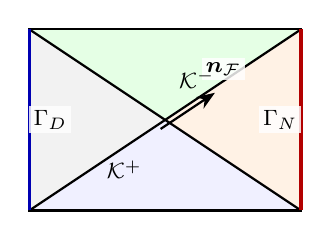
\begin{tikzpicture}[scale=1.15]
      \coordinate (A) at (0,0);
      \coordinate (B) at (3,0);
      \coordinate (C) at (3,2);
      \coordinate (D) at (0,2);
      \coordinate (E) at (1.5,1);
      \fill[blue!6] (A)--(B)--(E)--cycle;
      \fill[orange!10] (B)--(C)--(E)--cycle;
      \fill[green!10] (C)--(D)--(E)--cycle;
      \fill[gray!10] (D)--(A)--(E)--cycle;
      \draw[thick] (A)--(B)--(C)--(D)--cycle;
      \draw[thick] (A)--(E)--(B) (C)--(E)--(D);
      \draw[very thick,blue!70!black] (A)--(D);
      \draw[very thick,red!70!black] (B)--(C);
      \draw[-{Stealth},thick] (1.45,0.9)--(2.05,1.3);
      \node[font=\footnotesize,fill=white,fill opacity=0.82,text opacity=1,
        inner sep=1.5pt] at (0.23,1) {$\GamD$};
      \node[font=\footnotesize,fill=white,fill opacity=0.82,text opacity=1,
        inner sep=1.5pt] at (2.77,1) {$\GamN$};
      \node[font=\footnotesize,fill=white,fill opacity=0.82,text opacity=1,
        inner sep=1.5pt] at (2.14,1.56) {$\bn_{\mathcal F}$};
      \node[font=\footnotesize] at (1.05,0.45) {$\mathcal K^+$};
      \node[font=\footnotesize] at (1.85,1.45) {$\mathcal K^-$};
    \end{tikzpicture}
  \end{column}
  \begin{column}{0.50\textwidth}
    \begin{itemize}
      \item $\Fh^{\mathrm{int}}$: interior facets shared by two elements;
      \item $\Fh^D$: boundary facets on $\GamD$;
      \item $\Fh^N$: boundary facets on $\GamN$.
    \end{itemize}
    On an interior facet, label the neighboring elements $\mathcal K^+$ and
    $\mathcal K^-$. Choose $\bn_{\mathcal F}$ to point from
    $\mathcal K^+$ to $\mathcal K^-$. This fixes an orientation for the
    facet.

    \vspace{0.2cm}
    The next slide distinguishes a scalar jump from the complete normal-flux
    jump used in the residual.
  \end{column}
\end{columns}
\end{frame}

\begin{frame}{The normal-flux jump includes the chosen normal}
For a piecewise scalar quantity $w$, the oriented jump is
\[
  [\![w]\!]_{\mathcal F}=w^+-w^-.
\]
Reversing the element labels changes its sign:
\[
  w^--w^+=-[\![w]\!]_{\mathcal F}.
\]

For a piecewise vector field $\bm p$, the quantity needed after integration
by parts is the \textbf{normal-flux jump}
\[
  [\![\bm p\cdot\bn_{\mathcal F}]\!]_{\mathcal F}
  :=(\bm p^+-\bm p^-)\cdot\bn_{\mathcal F}.
\]
If the labels are reversed, the chosen normal must also be reversed. Therefore
\[
  (\bm p^--\bm p^+)\cdot(-\bn_{\mathcal F})
  =(\bm p^+-\bm p^-)\cdot\bn_{\mathcal F}.
\]
The two sign changes cancel. Only this complete normal-flux expression is
independent of the labeling.
\end{frame}

\begin{frame}{First local step: integrate by parts on one element}
The gradient term in the residual is a sum over elements:
\[
  \int_\Om k\grad u_h\cdot\grad v\,\dd x
  =\sum_e\int_{\mathcal K_e}k\grad u_h\cdot\grad v\,\dd x.
\]
On one element, Green's formula gives
\[
\begin{aligned}
 \int_{\mathcal K_e}k\grad u_h\cdot\grad v\,\dd x
 ={}&-\int_{\mathcal K_e}\divg(k\grad u_h)v\,\dd x\\
 &+\int_{\partial\mathcal K_e}
 (k\grad u_h\cdot\bn_e)v\,\dd s,
\end{aligned}
\]
where $\bn_e$ is the outward normal of $\mathcal K_e$.

\vspace{0.2cm}
This operation moves the derivative from $v$ onto the computed flux. It
creates an element-interior term and one boundary term for every element.
\end{frame}
\end{document}
